\documentclass[psamsfonts]{amsart}

%-------Packages---------
\usepackage{amssymb,amsfonts}
\usepackage[all,arc]{xy}
\usepackage{enumerate}
\usepackage{mathrsfs}
\usepackage{amsmath}
\usepackage{tikz}
\usepackage{mathtools}
\usepackage{float}
\usepackage{graphicx}

%--------Theorem Environments--------
%theoremstyle{plain} --- default
\newtheorem{thm}{Theorem}[section]
\newtheorem{cor}[thm]{Corollary}
\newtheorem{prop}[thm]{Proposition}
\newtheorem{lem}[thm]{Lemma}
\newtheorem{conj}[thm]{Conjecture}
\newtheorem{quest}[thm]{Question}

\theoremstyle{definition}
\newtheorem{defn}[thm]{Definition}
\newtheorem{defns}[thm]{Definitions}
\newtheorem{con}[thm]{Construction}
\newtheorem{exmp}[thm]{Example}
\newtheorem{exmps}[thm]{Examples}
\newtheorem{notn}[thm]{Notation}
\newtheorem{notns}[thm]{Notations}
\newtheorem{addm}[thm]{Addendum}
\newtheorem{exer}[thm]{Exercise}

\theoremstyle{remark}
\newtheorem{rem}[thm]{Remark}
\newtheorem{rems}[thm]{Remarks}
\newtheorem{warn}[thm]{Warning}
\newtheorem{sch}[thm]{Scholium}

\makeatletter
\let\c@equation\c@thm
\makeatother
\numberwithin{equation}{section}

\bibliographystyle{plain}

%--------Meta Data: Fill in your info------
\title{Applications of M\"{o}bius Inversion on Partially Ordered Sets}

\author{David Wu}

\begin{document}

\begin{abstract}
In this paper, we discuss how the theory of partially ordered sets plays an important role in  combinatorics. First, we outline definitions for partially ordered sets. Next, we introduce incidence algebra and M\'{o}bius inversion. Then, we present three applications of partially ordered set theory: the Inclusion-Exclusion Principle, Euler's Totient function (or phi function), and P\'{o}lya's Enumeration Theorem. For  P\'{o}lya's Enumeration Theorem, we assume prior knowledge of basic group theory.
\end{abstract}
\maketitle

\tableofcontents

\section{Introduction}
\indent Many problems in combinatorics deal with counting a particular combinatorial object. A common strategy is to construct an algebraic object to do this counting (ex. generating functions). In this paper, the combinatorial object of interest is the partially ordered set, and the algebraic object we use is incidence algebra. In particular, we are most interested in the Kronker delta, zeta, and M\"{o}bius function in incidence algebra. These functions give rise to a technique called the M\"{o}bius inversion formula, a counting tool with far-reaching applications. \\
\indent In section 2, we begin by introducing preliminary definitions for partially ordered sets. In section 3, we define incidence algebra and introduce the M\"{o}bius inversion formula. In section 4, we apply M\"{o}bius inversion to arrive at three well-known results, the finite version of the fundamental theorem of calculus, the Inclusion-Exclusion Principle, and Euler's Totient function. In the last section, we introduce a standard tool of enumerative combinatorial theory, P\'{o}lya's Enumeration Theorem, and present a proof using partially ordered sets and double M\"{o}bius inversion originally presented by Gian-Carlo Rota and David A. Smith in 1977\cite{Polya}. For this theorem, we assume prior knowledge of group theory including the symmetric group, group actions, orbits, and stabilizers.

\section{Basic Definitions for Partially Ordered Sets (Posets)}  
Partially ordered sets are powerful tools in algebraic combinatorics, as they bring structure to many problems where certain objects may not be comparable. 
\begin{defn}  
A \textit{partially ordered set} $P$ (or \textit{poset}) is a set (which we also denote $P$) equipped with a binary relation denoted $\leq_P$ (or $\leq$) satisfying the following three axioms:
\begin{enumerate}
    \item For all $x\in P$, $x \leq x$ (\textit{Reflexivity}).
    \item For all $x, y\in P$, if $x \leq y$ and $y\leq x$, then $x = y$ (\textit{Antisymmetry}).
    \item For all $x, y, z\in P$, if $x\leq y$ and $y\leq z$, then $x\leq z$ (\textit{Transitivity}).
\end{enumerate}
We say that two elements $x$ and $y$ of $P$ are \textit{comparable} if $x\leq y$ or $y\leq x$. Otherwise, $x$ and $y$ are \textit{incomparable}, which we denote $x\| y$.
\end{defn}

\begin{defn}
The \textit{dual} of a poset $P$ is the poset $P^*$ on the same set as $P$ but with reversed ordering. In other words, $x\leq y$ in $P^*$ if and only if $y\leq x$ in $P$. 
\end{defn}

\begin{defn}
An \textit{induced subposet} of $P$ is a subset $Q$ of $P$ and a partial ordering of $Q$ such that for $x,y\in Q$, $x\leq y$ in $Q$ if and only if $x\leq y$ in $P$.\\
A \textit{closed interval} $[x,y]$ is a subposet of P where $[x,y] = \{ z\in P \ | \ x\leq z \leq y\}$, defined whenever $x\leq y$.\\
If every interval of $P$ is finite, then $P$ is called a \textit{locally finite poset}.
\end{defn}
\begin{defn}
Given a poset $P$, if $x,y\in P$, we say $x$ \textit{covers} $y$ if $x<y$ and there does not exist an element $z\in P$ satisfying $x<z<y$.
\end{defn}

Many times, we work with posets where every element is comparable, which we call a \textit{total ordering}. We call these posets \textit{chains}. With this, we see that partial ordering generalizes total ordering.

\begin{defn}
A \textit{chain} is a poset in which any two elements are comparable. If $C$ is a chain and subposet of $P$, then $C$ is called \textit{maximal} if it is not contained in a larger chain of $P$. A \textit{multichain} of a poset $P$ is a chain with repeated elements. 
\end{defn}
\begin{defn}
The \textit{length} $\ell(C)$ of a finite chain $C$ is defined by $\ell(C) = \#C - 1$. The \textit{length} (or \textit{rank}) of a finite poset $P$ is
\begin{equation*}
    \ell(P) := max\{\ell(C) \ | \ C \text{ is a chain of } P\}.
\end{equation*}
\end{defn}

\begin{defn}
An \textit{order ideal} of a poset P is a subset $I$ of $P$ satisfying:
\begin{enumerate}
    \item $I$ is non-empty.
    \item For every $x$ in $I$, if $y$ is in $P$ and $y\leq x$, then $y$ is in $I$.
    \item For every $x,y$ in $I$, there is some $z$ in $I$ such that $x\leq z$ and $y\leq z$.
\end{enumerate}
Given an element $x$ in $P$, the \textit{principal order ideal} generated by $x$ is the set defined as $\Lambda_x=\{y\in P \mid y \leq x\}$.
\end{defn}

\begin{defn}
The \textit{direct product} of posets $P$ and $Q$ is the poset $P\times Q$ on the set $\{(x,y) \ | \ x\in P, y\in Q\}$ such that $(x,y)\leq (x',y')$ in $P\times Q$ if $x\leq_P x'$ in $P$ and $y\leq_Q y'$ in $Q$.
\end{defn}

\begin{defn}
An \textit{upper bound} of elements $x$ and $y$ in a poset $P$ is an element $z\in P$ such that $z\geq x$ and $z\geq y$. 
A \textit{lower bound} of elements $x$ and $y$ in a poset $P$ is an element $z\in P$ such that $z\leq x$ and $z\leq y$.
\end{defn}

\begin{defn}
Let $P$ be a poset with elements $x$ and $y$.\\
An element $z$ of $P$ is the join of $x$ and $y$, denoted $x\vee y$, if 
\begin{enumerate}
    \item $z\geq x$ and $z\geq y$.
    \item For any $w\in P$ such that $w\geq x$ and $w\geq y$, we have $w\geq z$.
\end{enumerate}
An element $z$ of $P$ is the meet of $x$ and $y$, denoted $x\wedge y$, if 
\begin{enumerate}
    \item $z\leq x$ and $z\leq y$.
    \item For any $w\in P$ such that $w\leq x$ and $w\leq y$, we have $w\leq z$.
\end{enumerate}
If the join and/or meet of $x$ and $y$ exists, then they are unique.
\end{defn}

\begin{defn}
  A poset $P$ has a \text{least element} which we denote $\hat{0}\in P$ if for all $x\in P$, $x\geq \hat{0}$. Similarly, $P$ has a \text{greatest element} which we denote $\hat{1}$ if for all $x\in P$, $x\leq \hat{1}$. 
\end{defn}
\begin{defn}
A \textit{lattice} $L$ is a poset where every pair of elements has a join and a meet. All finite lattices have a $\hat{0}$ and $\hat{1}$. 
\end{defn}

\begin{rem}
We can draw finite posets as a graph called a \textit{Hasse Diagram}, where the vertices are elements and the edges are cover relations. If $x,y\in P$ and $x<y$, then we draw $x$ below $y$ in the Hasse Diagram. 
\end{rem}
\begin{exmp}\label{Hasse example}
The Hasse diagram for the elements of the power set of $\{1,2\}$ ordered by inclusion (if $A, B \in P$ then $A\leq B$ if and only if $A\subseteq B$) is
\[
\xymatrix{
  & \{1,2\} \ar@{-}[dr] \ar@{-}[dl] \\
  \{1\} \ar@{-}[dr] & & \{2\} \ar@{-}[dl] \\
  & \emptyset}
\]
\end{exmp}


\section{Incidence Algebra}
 \textit{Incidence algebra} provides a framework for inversion with the \textit{M\"{o}bius Function}. Let $P$ be a locally finite poset, and let $Int(P)$ be the set of closed intervals of $P$. Let $K$ be a field. For mappings $f:Int(P)\rightarrow K$, denote $f([x,y])$ as $f(x,y)$. 
\begin{defn}
The \textit{incidence algebra} $I(P,K)$ (or $I(P)$) of $P$ over $K$ is the $K-algebra$ over the vector space of all functions
\begin{equation*}
    f: Int(P) \rightarrow K
\end{equation*}
where we define addition and scaler multiplication pointwise, and multiplication $*$ as \textit{convolution} defined by
\begin{equation*}
    (f * g)(a,c) = fg(a,c) = \sum_{a\leq b\leq c}f(a,b)g(b,c).
\end{equation*}
Because $P$ is locally finite, the above sum is finite, so $fg$ is well-defined.
\end{defn}

There are three key functions from incidence algebra, which we detail below.

\begin{defn}
$I(P,K)$ is an associative algebra with a two-sided identity \\$\delta\in I(P,K)$ called the \textit{Kronecker delta function} defined
\begin{equation}\label{delta_function}
    \delta(x,y) = 
    \begin{cases}
    1 & \text{if } x = y\\
    0 & \text{if } x\neq y
    \end{cases}
\end{equation}
\end{defn}

\begin{defn}
The \textit{zeta function} $\zeta \in I(P,K)$ is defined
\begin{equation}\label{zeta_function}
    \zeta(x,y) =
    \begin{cases}
    1 & x\leq y\\
    0 & \text{otherwise}
    \end{cases}
\end{equation}
The zeta function is very useful for counting chains. Given an interval $(x,y)$, the number of multichains of length $n$ from $x$ to $y$ can be found using
\begin{equation*}\displaystyle\zeta^{n}(x,y)=\sum_{x=x_0\leq x_1,\leq \dots \leq s_n=y} 1,
\end{equation*} 
Similarly, the equation
\begin{equation*}
    (\zeta - 1)(x,y) = 
    \begin{cases}
    1 & \text{if $x < y$}\\
    0 & \text{if $x=y$}
    \end{cases}
\end{equation*}
counts the number of chains $x=x_0<x_1<\dots<x_n=y$ of length $n$ from $x$ to $y$. 
\end{defn}

\begin{prop}
The zeta function has an inverse $\mu$ called the \textit{M\"{o}bius Function} defined recursively as
\begin{equation}\label{mobius_function}
    \begin{array}{l}
    \mu(x,x)=1 \text{ for all } x\in P \\ 
    \mu(x,y)=-\displaystyle\sum_{x\leq z < y}\mu(x,z) \text{ for all } x<y \text{ in P.}\\
  \end{array}
\end{equation}
\begin{proof}
If $\mu$ is the inverse of $\zeta$ then $\mu\zeta = \delta$. Using induction over the number of elements in $[x,y]$, let $\mu(x,x)=1$ for all $x\in P$ and assume $\mu(x,z)$ is defined for all $z$ in the interval $[x,y)$. Then
\begin{equation}
\mu\zeta(x,y)=\delta(x,y) \iff \sum_{x\leq z \leq y}\mu(x,z)\zeta(z,y)=0 \iff \mu(x,y)+\sum_{x\leq z < y}\mu(x,z)=0 
\end{equation}
meaning $\mu(x,y)=-\displaystyle\sum_{x\leq z < y}\mu(x,z)$ if $x<y$ as desired. 
\end{proof}
\end{prop}
\begin{cor}
 From the definition of the M\"{o}bius Function, 
\begin{equation}\label{mobius_delta}
\sum_{z\leq y\leq x}\mu(y,x)=\delta(z,x)
\end{equation}
\end{cor}

\begin{rem}
If $Q$ be a non-empty subset of $P$, with the induced order, then we can consider $I(Q,k)$ as a \textit{subalgebra} (where the operation is closed in $Q$) of $I(P,K)$. 
\end{rem}

The following result is fundamental to many of the enumeration problems we will encounter in this paper.

\begin{thm} [M\"{o}bius inversion formula]
Let $P$ be a poset for which every principal order ideal is finite. Define functions $f,g:P\to K$. Then
\begin{equation}\label{mobius_inversion_1}
    f(x)=\sum_{y\leq x}g(y) \text{ for all $x\in P$}
\end{equation}
if and only if
\begin{equation}\label{mobius_inversion_2}
    g(x)=\sum_{y\leq x}f(y)\mu(y,x) \text{ for all $x\in P$}
\end{equation}
\begin{proof}
Assume (\ref{mobius_inversion_1}) is true. Let $x\in P$ be arbitrary. Substitute the right side of (\ref{mobius_inversion_1}) into the right side of (\ref{mobius_inversion_2}) to get
\[
\sum_{y\leq x}f(y)\mu(y,x) = \sum_{y\leq x}\sum_{z\leq y}g(z)\mu(y,x)=\sum_{y\leq x}\sum_{z\leq y}g(z)\zeta(z,y)\mu(y,x).
\]
By interchanging the order of the summation, we get
\[
=\sum_{z\leq x}g(z)\sum_{z\leq y\leq x}\zeta(z,y)\mu(y,x)=\sum_{z\leq x}g(z)\delta(z,x)=g(x).
\]
Now assume (\ref{mobius_inversion_2}) is true. Let $x\in P$ be arbitrary. Substitute the right side of (\ref{mobius_inversion_2}) into the right of (\ref{mobius_inversion_1}) to get
\[
\sum_{y\leq x}g(y)=\sum_{y\leq x}g(y)\zeta(y,x)=\sum_{y\leq x}\sum_{z\leq y}f(z)\mu(z,y)\zeta(y,x)
\]
By interchanging the order of the summation, we get
\[
=\sum_{z\leq y} f(z)\sum_{z\leq y\leq x}\mu(z,y)\zeta(y,x)=\sum_{z\leq x}f(z)\delta(z,x)=f(x)
\]
\end{proof}
\end{thm}
\begin{rem}
In essence, M\"{o}bius Inversion is the statement
\begin{equation}
    g\zeta=f\iff g=f\mu.
\end{equation}
\end{rem}

\indent Before we move on to applications, we prove one more statement to allow us to apply M\"{o}bius inversion on the direct product of finite posets.

\begin{thm}[Product Theorem]\label{Product Theorem}
Let $P$ and $Q$ be locally finite posets with the direct product $P\times Q$. If $(x,y)\leq (x',y')$ in $P\times Q$ then
\begin{equation}
    \mu_{P\times Q}((x,y),(x',y'))=\mu_P(x,x')\mu_Q(y,y').
\end{equation}
\begin{proof}
If $(x,y)\leq (x',y')$, then 
\begin{align*}
    \sum_{\mathclap{(x,y)\leq (u,v)\leq (x',y')}} \mu_P(x,u)\mu_Q(y,v)&= \left(\sum_{x\leq u \leq x'}\mu_P(x,u)\right)\left(\sum_{y\leq v \leq y'}\mu_Q(y,v)\right)\\
    &= \delta_{xx'}\delta_{yy'}\\
    &=\delta_{(x,y),(x',y')}.
\end{align*}

This matches (\ref{mobius_delta}). Since $\mu$ is uniquely determined, the proof is complete.
\end{proof}
\end{thm}

\section{Applications of M\"{o}bius inversion}
\indent M\"{o}bius Inversion is a sieving procedure, where we overcount items and remove items that we don't need. One of the most fundamental examples of M\"{o}bius inversion results in a simplification of Inclusion-Exclusion. First, we will explore how to derive M\"{o}bius functions for certain posets in order to use M\"{o}bius inversion.
\begin{exmp}[Natural Number Chain]\label{natural_chain}
Let $P$ be the chain $\mathbb{N}$. Then the M\"{o}bius function immediately follows from (\ref{mobius_function}).
\[
\mu(x,y)=\begin{cases}
1 & \text{ if } x=y\\
-1 & \text{ if } x+1=y\\ 
0 & \text{ otherwise}.
\end{cases}
\]
The M\"{o}bius inversion formula immediately follows from (\ref{mobius_inversion_1}) and (\ref{mobius_inversion_2}).
\[
f(n)=\sum^n_{k=0}g(k) \text{ for all $n>0$ }
\]
if and only if 
\[
g(0)=f(0) \text{ and } g(n)=f(n)-f(n-1) \text{ for all } n>0.
\]
One may recognize this as the finite version of the \textit{fundamental theorem of calculus}. Here, the M\"{o}bius function acts as the $\Delta$ operator, which has an inverse $\Sigma$. 
\end{exmp}
\subsection{Inclusion-Exclusion Principle} \hfill\\
\indent The \textit{Inclusion-Exclusion Principle} is one of the most important results in counting. Here, we will see how M\"{o}bius inversion on a poset called the \textit{Boolean Lattice} (or \textit{Boolean Algebra}) is equivalent to the Inclusion-Exclusion Principle.

\begin{defn}[Boolean lattice]
 Given a set $S$ and its powerset $2^n$ where $n=\#S$, we define a \textit{Boolean lattice} (or \textit{Boolean algebra}) of \textit{rank} $n$, where the elements are subsets of $S$ and the ordering is defined by \textit{inclusion} (if $A,B\subseteq S$, then $A\leq B$ if and only if $A\subseteq B$). A \textit{Boolean lattice} is a distributive lattice (join and meet distribute) where every element has a complement. We denote the lattice as $B_n$. (\ref{Hasse example}) is an example of a Boolean lattice.
\end{defn}
Now we will calculate the M\"{o}bius function for a Boolean lattice. For the following results, let $P=B_n$, the Boolean lattice of rank $n$. 

\begin{prop}\label{mobius_bl}
Let $S,T\subseteq P$. Then the M\"{o}bius function for $P$ is 
\begin{equation}
\mu(S,T) = 
\begin{cases}
(-1)^{\#T-\#S} & \text{if } S\subseteq T\\
0 & \text{otherwise}
\end{cases}
\end{equation}
\begin{proof}
Let $\mathbf{2}=\{0,1\}$ be a chain of two elements. We can think of $B_n$ as the set of all subsets of an n-sized set $A$. So, for a subset $S$ of $A$, we can think of the elements of $A$ mapping to $1$ if they are in $S$, and $0$ if not. Hence, $B_n$ is isomorphic to the product $\mathbf{2}^n$, the set of $n$-tuples of 0's and 1's. By example \ref{natural_chain}, the M\"{o}bius function for $\mathbf{2}$ is $\mu(0,0)=\mu(1,1)=1$, $\mu(0,1)=-1$. By the product theorem, for $n$-tuples $S=(s_1,...,s_n)$ and $T=(t_1,...,t_n)$, 
\[
\mu((s_1,...s_n),(t_1,...,t_n))=\displaystyle\prod^n_{i=1}\mu(s_i,t_i)=(-1)^{\mathbf{2}^{t_i}-\mathbf{2}^{s_i}}=(-1)^{\#T-\#S}
\]
\end{proof}
\end{prop}
The Inclusion-Exclusion principle follows from  M\"{o}bius inversion on $B_n$. 
\begin{thm}[Inclusion-Exclusion Principle]
Suppose we have $N$ items and a collection of $k$ properties $P=\{p_1,p_2,\dots, p_n\}$. Let $N_i$ be the number of items that satisfy $P_i$, $N_{ij}$ the number of items that satisfy properties $P_i$, and $P_j$ and so on. Then the number of items that satisfy none of these properties, $N_0$ is
\begin{equation*}
    N_0= N - \sum N_i+\sum_{i_1<i_2}N_{i_1i_2}-\sum_{i_1<i_2<i_3}N_{i_1i_2i_3}+\dots + (-1)^nN_{12\dots n}.
\end{equation*}
\begin{proof}
Let $T$ be a collection of properties. Define the function $g(T)$ to be the number of items which satisfy exactly the properties in $T$ and no others. Define the function $f(T)$ to be the number of items which satisfy every property in $T$ and possibly others. Then  
\[
f(T)=\sum_{S\subseteq T}g(S).
\]
By M\"{o}bius inversion, 
\[
g(T)=\sum_{S\subseteq T}f(S)(-1)^{\#T-\#S}.
\]
The above equation is the Inclusion-Exclusion principle. To find $N_0$, let $g(\emptyset)=N_0$ and $f(\emptyset)=N$. Then 
\begin{equation*}
    f(\emptyset)-g(\emptyset) = \sum_{T\neq \emptyset}(-1)^{\#T-1}f(T)
\end{equation*}
This equation gives the number of items which satisfy at least one property, or  the union if thinking in terms of sets. Therefore the number of elements that satisfy no properties, or $N_0$, is
\begin{equation*}
    N_0=g(\emptyset)=f(\emptyset)+\sum_{T\neq \emptyset}(-1)^{\#T}f(T)
\end{equation*}
\end{proof}
\end{thm}
\subsection{Classical M\"{o}bius Function} \hfill\\
\indent The M\"{o}bius function was first introduced in 1832 by August Ferdinand M\"{o}bius in the field of number theory as the \textit{Classical M\"{o}bius Function}. The Classical M\"{o}bius Function arises as the M\"{o}bius function for the poset of divisors of an integer $n$, $D_n$. By using M\"{o}bius inversion on $D_n$, we can derive \textit{Euler's phi function} (or \textit{Euler's Totient function}).

\begin{defn}
Let $D_n$ denote the poset of consisting of integer divisors of a positive integer $n$. $D_n$ is ordered by divisibility such that $x\leq y$ if and only if $x\vert y$.
\end{defn}

\begin{prop}
The M\"{o}bius function for $D_n$ is 
\begin{equation}
    \mu(x,y) = \begin{cases}
    (-1)^t & \text{if $\frac{y}{x}$ is a product of t distinct primes}\\
    0 & otherwise.
    \end{cases}
\end{equation}
\begin{proof}
 Let $P=(\mathbf{k_1 + 1})\times (\mathbf{k_2 + 1}) \times \dots \times (\mathbf{k_n + 1})$ be the product of chains of lengths $k_1, \dots, k_n$. By Example \ref{natural_chain} and Theorem \ref{Product Theorem}, for n-tuples $(a_1,\dots, a_n)$ and $(b_1, \dots, b_n)$, we have
 \begin{equation*}
     \mu((a_1,\dots, a_n),(b_1, \dots, b_n))=\begin{cases}
     (-1)^{\sum(b_i-a_i)} & \text{if each $b_i-a_i=0$ or $1$}\\
     0 & \text{otherwise}.
     \end{cases}
 \end{equation*}
 Consider the poset $D_n$ of divisors of a positive integer $n$. Suppose $n$ has the prime factorization $p_!^{k_1}p_1^{k_2}\dots p_n^{k_n}$. We can think of each $p_i^{k_i}$ as the poset $D_{p_i^{k_i}}$, the chain \[1<p_i^1<p_i^2<\dots <p_i^{k_i}.\]
 It follows that \[D(n)\cong D(p_1^{k_1})\times D(p_2^{k_2}) \times \cdots\times D(p_n^{k_n}).\]
 If we substitute each $k_i$ in $P$, we see $D_n\cong P$. Thus, 
 \begin{equation}
     \mu(x,y) = \begin{cases}
    (-1)^t & \text{if $\frac{y}{x}$ is a product of t distinct primes}\\
    0 & \text{otherwise}
    \end{cases}
 \end{equation}
 as desired.
\end{proof}
\end{prop}
\begin{rem}
$\mu(x,y)$ is the same as the number-theoretic M\"{o}bius function $\mu(\frac{y}{x})$, which is
\begin{equation}
    \mu(n) = \begin{cases}
    1 & \text{if $n=1$}\\
    (-1)^k & \text{if $n$ is a product of $k$ distinct primes}\\
    0 & \text{if $n$ has one or more repeated prime factors}.
    \end{cases}
\end{equation}
\end{rem}
\begin{defn}\label{euler phi}
\textit{Euler's phi function} (or \textit{Euler's Totient function}) counts the number of positive integers k less than $n$ that are \textit{relatively prime} to n, i.e $\gcd(n,k)=1$ with the following equation:
\begin{equation}
    \varphi(n) = n\prod_{p\vert n}\left(1-\frac{1}{p}\right),
\end{equation}
where the product ranges over all distinct prime numbers $p$ dividing $n$. 
\end{defn}

To derive Euler's phi function, we first introduce some number theoretic results. 

\begin{lem}\label{divide by GCD}
Two numbers divided by their GCD are relatively prime to each other, i.e. if $gcd(a,b)=d$ then $gcd(\frac{a}{d},\frac{b}{d})=1$.
\end{lem}
\begin{proof}
Let $gcd(a,b)=d$. Suppose for contradiction that $gcd(\frac{a}{d}.\frac{b}{d})=c$ where $c>1$. Then $cd\vert a$ and $cd \vert b$, so $cd$ is a divisor of $a$ and $b$. But since $c>1$, we have that $cd>d$. Thus, $c$ would not be the gcd of $a$ or $b$, which is a contradiction. 
\end{proof}

\begin{lem}\label{phi sum = n}
For a positive integer $n$, 
\begin{equation*}
    \sum_{d\vert n} \varphi(d) = n.
\end{equation*}
\begin{proof}
Let $n$ be a positive integer and define the set $[n]=\{1,2,\dots,n\}$. Partition $[n]$ into sets $S_d$ such that $S_d=\{m\in \mathbb{Z} \mid 1\leq m \leq n, \gcd(m,n)=d\}$ where each $S_d$ represents all the numbers less than or equal to $n$ whose GCD with $n$ is $d$. From this construction, for all $1\leq m \leq n$, there exists some $d$ such that $dm = n$. Furthermore, each $S_d$ are disjoint, so the union of all $S_d$ is $[n]$. Hence,
\[
    n = \sum_{d\vert n} \#S_d.
\]
By lemma \ref{divide by GCD}, for any $m\in S_d$, there exists some $k\in \mathbb{Z}$ such that $m=kd$ and $\gcd(k,\frac{n}{d})=1$. Then $\#S_d=\varphi(\frac{n}{d})$, meaning  
\[
    n = \sum_{d\vert n} \#S_d = \sum_{d\vert n} \varphi(d).
\]
\end{proof}
\end{lem}

\begin{prop}
M\"{o}bius inversion with the Classical M\"{o}bius function yields Euler's phi function. 
\begin{proof}
From lemma \ref{phi sum = n} and definition \ref{euler phi}, we have the result
\[
n=\sum_{d\vert n}\varphi(d).
\]
To find $\varphi(n)$, we use M\"{o}bius inversion and get
\begin{equation}
    \varphi(n)=\sum_{d\vert n}\mu\left(\frac{n}{d}\right)d=n-\frac{n}{p_1}-\frac{n}{p_2}-\cdots + \frac{n}{p_1p_2}+\cdots,
\end{equation}
as $\mu(\frac{n}{d})$ is non-zero if and only if $\frac{n}{d}$ is a product of distinct primes $p_i$. Thus, 
\begin{equation*}
    \varphi(n) = n\prod_{p\vert n}\left(1-\frac{1}{p}\right)
\end{equation*}
where $p$ is a prime dividing $n$.
\end{proof}
\end{prop}

\section{P\'{o}lya's Enumeration Theorem}
\indent Suppose we have a set of objects and a set of colorings. By representing the objects as groups of symmetries, we can enumerate equivalence classes of colorings to solve for configurations of object colorings with \textit{P\'{o}lya's Enumeration Theorem}. In this paper, we will present a proof  utilizing posets and M\"{o}bius inversion presented by Gian-Carlo Rota and David A. Smith in 1977\cite{Polya}. First, we will introduce preliminary definitions. Next, we will establish a Galois connection between a lattice of permutations and a lattice of partitions of the set the permutation group acts on. Then, we will introduce appropriate formal power series as generating functions for sets of colors. Lastly, we will perform computations on the smaller lattices and transfer them back to the larger ones. 


\begin{defn}
Let $G$ be a group. Two group elements $h,k\in G$ are \textit{conjugate} if there is an element $g\in G$ such that $k=g^{-1}hg$. This is an equivalence relation whose equivalence classes are called \textit{conjugacy classes}. Subgroups $H,K\leq G$ are \textit{conjugate subgroups} if $K=g^{-1}Hg$ for some $g\in G$. Here, $g^{-1}Hg$ is the set of elements $g^{-1}hg$ for $h\in H$. 
\end{defn}

\begin{thm}\label{conjugate subgroup orbits}
Let $G$ be a group and $X$ be a $G-$set. Suppose $x$ and $y$ are in the same orbit. Then the stabilizer groups $G_x$ and $G_y$ are conjugate subgroups. 
\begin{proof}
Because $x$ and $y$ are in the same orbit, there is a group element $g\in G$ such that $y=gx$. Then for $h\in G_y$, $h(gx)=gx$. Applying $g^{-1}$ to both sides yields $(g^{-1}hg)x=x$, so $g^{-1}hg\in G_x$. 
\end{proof}
\end{thm}

\begin{defn}
A \textit{partition} $\pi$ of a finite $n$ element set $S$ is a collection $\{\pi_1,\pi_2,\dots\}$ of non-empty, mutually disjoint subsets of $S$ whose union is $S_n$. The sets $\pi_i$ are called the \textit{blocks} of $\pi$. 
\end{defn}

\begin{rem}
For any equivalence relation on a set $X$, the set of its equivalence classes is a partition of $X$. From any partition $\pi$ of $X$, we can define an equivalence relation on $X$ by letting $x\sim y$ if $x$ and $y$ are in the same block in $\pi$. Thus, equivalence relations and partitions are analogous.
\end{rem}

\begin{defn}
Given two partitions $\pi$ and $\sigma$, we say $\pi$ is a \textit{refinement} of $\sigma$ if every block $\pi_i\in \pi$ is contained in some block $\sigma_i\in \sigma$. 
\end{defn}

\begin{defn}\label{kernel} Let $X$ and $Y$ be sets and let $f$ be a function $f:X\to Y$. The \textit{kernel} of the function $f$ is the equivalence relation on the domain $X$ defined as follows, elements $x_1$ and $x_2$ in $X$ are \textit{equivalent} if $f(x_1)$ and $f(x_2)$ map to the same element in $Y$. It follows that the kernel forms a partition of $X$. 
\end{defn}


\begin{defn}
A \textit{closure operator} (or \textit{closure relation}) in a poset $P$ is a function $x\to \overline{x}$ of $P$ into itself with the properties
\begin{enumerate}
    \item $\overline{x}\geq x$.
    \item $\overline{\overline{x}}=\overline{x}$.
    \item $x\geq y$ implies $\overline{x}\geq \overline{y}$
\end{enumerate}
In other words, these are idempotent, increasing mappings. An element is \textit{closed} if $x=\overline{x}$.
\end{defn}

\begin{defn}\label{galois connection}
Let $P$ and $Q$ be two posets. A \textit{Galois connection} between $P$ and $Q$ is a pair of functions $\theta:P\to Q$ and $\eta: Q\to P$ satisfying 
\begin{enumerate}
    \item Both $\theta$ and $\eta$ are order-inverting.
    \item For $p\in P$, $\eta(\theta(p))\geq p$.
    \item For $q\in Q$, $\theta(\eta(q))\geq q$.
\end{enumerate}
The mappings $p\to \eta(\theta(p))$ and $q\to \theta(\eta(q))$ are closure operators, and the two posets formed by the closed sets are isomorphic. 
\end{defn}
\subsection{A Galois connection between permutations and partitions}\hfill\\
\indent Let $G$ be a group of permutations of a set $S$ and define $L(G)$ to be the lattice of subgroups of $G$ ordered by inclusion. Define $\Pi(S)$ to be the lattice of partitions of $S$ ordered by refinement.

\indent Define the mapping $\eta : L(G)\to \Pi(S)$ such that if $H$ is a subgroup of $G$, then $\eta(H)$ is the partition whose blocks are the $H$-orbits in $S$, or with the equivalence relation $x\sim y$ if and only if there is some $g\in H$ such that $gx=y$. This partition is called the \textit{period} of $H$.

\indent Define the mapping $\theta:\Pi(S)\to L(G)$ such that if $\pi$ is a partition of $S$, $\theta(\pi)$ is the set of group elements $g$ that leave the blocks of $\pi$ invariant, or the elements $g$ where the cycles of $g$ are contained within the blocks of $\pi$. Thus, $\theta(\pi)$ is a subgroup of $G$.

\begin{lem}
$\eta$ and $\theta$ are increasing mappings and 
\begin{equation}\label{thetaeta}
    H\leq \theta\eta(H) \text{ for all } H\in L(G)
\end{equation}
\begin{equation}\label{etatheta}
    \pi\geq \eta\theta(\pi) \text{ for all } \pi\in \Pi(S)
\end{equation}
\end{lem}
\indent One can verify  (\ref{thetaeta}) by noting that $\eta(H)$ maps to a partition such that $\theta$ is satisfied for more group elements than in $H$. (\ref{etatheta}) follows as $\theta(\pi)$ maps to a set of group elements which $\eta$ maps to a refined partition of $\pi$, as $\pi$ holds contains more cycles than its refinement.\\
\indent If we take the lattice $\Pi(S)^*$ dual to $\Pi(S)$, we see that $(\eta, \theta)$ satisfy Definition \ref{galois connection} and form a Galois connection on $L(G)$ and $\Pi(S)^*$. Then $\theta\eta$ and $\eta\theta$ form the closure operators on $L(G)$ and $\Pi(S)^*$ respectively. We call closed subgroups of $G$ \textit{periodic} and closed partitions of $S$ \textit{periods} (the partitions which are periods of subgroups of $G$). We denote a period $\eta\theta(\pi)$ as $\overline{\pi}$. From equation \ref{etatheta}, $\overline{\pi}$ is a refinement of $\pi$.
Define the lattice of periods of $G$ in $S$, $\text{Pers}(G,S)$, with induced refinement ordering as
\begin{equation*}
    \text{Pers}(G,S)=\{\pi \in \Pi(S) \mid \overline{\pi}=\pi\}.
\end{equation*}
\indent It is important to note that this may not be a sublattice of $\Pi(S)$ due to the ordering. By the definition of a Galois connection, $\eta$ and $\theta$ are inverse order isomorphisms between the lattice of periodic subgroups of $G$ and $\text{Pers}(G,S)$.

\subsection{Generating Functions}\hfill\\
\indent From the previous section, we established our set $S$ of objects, which we assume to be finite, and the group $G$ of symmetries that act on $S$. Now we introduce the notion of coloring. Let $X$ be a set of colors, at most countable. The set of colorings of $S$, denoted $X^S$, contains the functions $f:S\to X$. By Definition \ref{kernel}, the kernel of each $f\in X^S$ forms a partition of $S$. Call the closure of $\ker(f)$ the $G$-period of $f$ in $S$ and denote it as $\text{Per}(f)$. By the definition of $\theta$, we have
\begin{equation}
    \theta(\ker(f))=\{g\in G \mid fg=f\}
\end{equation}
where $\text{Per}(f)$ is the partition whose blocks are the orbits of $\theta(\ker(f))$.\\
\indent For each $f\in X^S$, we want to be able to label each ordered pair of object and color. For this, we associate with each $f\in X^S$ a monomial
\begin{equation*}\label{generating function 1}
    M(f)=\prod_{i\in S}x^{i}_{f(i)}.
\end{equation*}
Now we can express any set of colorings $A$ with a \textit{generating function}
\begin{equation*}\label{generating function 2}
    M(A)=\sum_{f\in A}M(f),
\end{equation*}
which is a formal power series in the indicated variables.

 \indent We call a set $F$ of functions a \textit{proper class} with respect to $G$ if $fg\in F$ whenever $f\in F$ and $g\in G$. Given a fixed proper class $F$ and a partition $\pi$ of $S$, we define the following generating functions:
\begin{equation}\label{generating function N=}
    N_{=}(\pi) = M(\{f\in F \mid \ker(f)=\pi\}),
\end{equation}
\begin{equation}\label{generating function NG=}
    N_{G=}(\pi)=M(\{f\in F \mid \text{Per}(f)=\pi\}),
\end{equation}
\begin{equation}\label{generating function N>=}
    N_{\geq}(\pi)=M(\{f\in F \mid \ker(f)\geq\pi\}).
\end{equation}
$N_{=}, N_{G=}, \text{ and } N_{\geq}$ are all functions on $\Pi(S)$ with values in $R[[x]]$, the ring of formal power series in the variables $x^{(i)}_j$.\\ 
\indent Define $M$ to be the additive group of functions $\Pi(S)\to R[[x]]$, and $I(\Pi(S),R[[x]])$ the incidence algebra of $\Pi(S)$ over $R[[x]]$. Thus, $M$ is a left and right module over $I(\Pi(S),R[[x]])$ such that if $k\in I(\Pi(S),R[[x]])$ and $A\in M$,
\begin{equation*}
kA(\pi)=\sum_{\sigma \geq \pi}k(\pi,\sigma)A(\sigma),
\end{equation*}
\begin{equation*}
    Ak(\pi)=\sum_{\sigma \leq \pi}A(\sigma)k(\sigma,\pi).
\end{equation*}
Let $\delta$, $\zeta$, and $\mu$ denote the delta, zeta, and M\"{o}bius function of $I(\Pi(S),R[[x]])$. The incidence algebra of $\text{Pers}(G,S)$ is a subalgebra of  $I(\Pi(S),R[[x]])$ with functions $\delta_P$, $\zeta_P$, and $\mu_P$. We define the function
\begin{equation}
    \overline{\delta}(\pi,\sigma)=\delta(\pi,\overline{\sigma}) \text{ for } \pi, \sigma\in \Pi(S).
\end{equation}

\begin{lem}\label{generating functions lemma 1}
Let $P$ be a poset and $Q$ be a subalgebra of $P$. Then \begin{equation}
    \overline{\delta}=\mu_{Q} \zeta
\end{equation} 
where $\mu_{Q}$ is the M\"{o}bius function on $Q$. 
\begin{proof}
Let $x,y\in P$. Then 
\begin{align*}
\overline{\delta}(x,y)&=\delta(x,\overline{y}) \\
&=\sum_{x\leq z\leq \overline{y}}\mu_Q(z,y) \text{ where $z$ is closed} \\
&=\sum_{x\leq z \leq y}\mu_Q(z,y)\\
&=\mu_Q\zeta(x,y)
\end{align*}
since non-zero terms in the sums can occur only for closed $z$, in which case $z\leq y$ if and only if $z\leq \overline{y}$.  
\end{proof}
\end{lem}

\begin{lem}\label{generating functions lemma 2}
From equations (\ref{generating function N=}) and (\ref{generating function N>=}), it follows immediately that
\begin{equation}
    N_{\geq}=\zeta N_{=}.
\end{equation}
\end{lem}
The following theorem relates the equations (\ref{generating function N=}), (\ref{generating function NG=}), and (\ref{generating function N>=})

\begin{thm}\label{theorem 1}
For any proper class $F$, 
\begin{equation}
    N_{G=}=\mu_P N_{\geq}= \overline{\delta} N_{=}.
\end{equation}
i.e. for any $\pi\in \Pi(S)$, 
\begin{equation}
    N_{G=}(\pi)=\sum_{\sigma\geq\pi}\mu_P(\pi,\sigma)N_{\geq}(\sigma)=\sum_{\overline{\tau}=\pi} N_{=}(\tau).
\end{equation}
\begin{proof}
By (\ref{generating function N=}) and (\ref{generating function NG=}),
\begin{align*}
    N_{G=}(\pi) &= \sum_{\text{Per}(f)=\pi}M(f)\\
    &=\sum_{\overline{\tau}=\pi}\left(\sum_{\ker(f)=\tau}\right)M(f)\\
    &=\sum_{\overline{\tau}=\pi}N_{=}(\tau).
\end{align*}

By lemma (\ref{generating functions lemma 1}) and (\ref{generating functions lemma 2}), $N_{G=}=\overline{\delta} N_{=} = \mu_P \zeta N_{=} = \mu_P N_{\geq}$. 
\end{proof}
\end{thm}

Now we will introduce two counting functions, a generalization of Euler's totient function (\ref{euler phi}) and a closely related function to perform M\"{o}bius inversion with.
For each period $\pi$, let
\begin{equation}\label{v function}
    v(\pi)=\#\theta(\pi).
\end{equation}
$v$ counts the number of group elements $g$ whose cycles are contained in blocks of $\pi$. Let
\begin{equation}
    \varphi(\pi)=\#\{g\in G \mid \text{cycles of $g$ are blocks of $\pi$}\}.
\end{equation}
\indent We can extend this to all of $\Pi(S)$ by defining $v$ and $\varphi$ to be $0$ if $\pi$ is not a period. Then we can think of them as elements of the module $M$ by identifying their values (integers) with constant power series. Furthermore, from their definitions, we see that they can be used for M\"{o}bius inversion.
\begin{equation}\label{v phi equation}
    v=\varphi \zeta_P \text{ and } \varphi = v \mu_P.
\end{equation}

\subsection{Proof of P\'{o}lya's Enumeration Theorem}\hfill

In this section, we will perform computations on our smaller lattice of closed partitions and transfer them back to the larger lattice of permutation subgroups. With the equations and generating functions from the previous section, we will explore their relationships and derive a generating function for equivalence classes of functions under a group action. Then, we will reformulate this in terms of group elements and arrive at a generalization of P\'{o}lya's Enumeration Theorem.

Let $F$ be our fixed proper class of functions $f:X\to S$, which can be thought of as admissible colorings. The group $G$ acts on $F$ by composition, i.e. $f\to fg$. The orbit of $f$ under this action is denoted $fG$. First, we introduce two lemmas that rely on permutation group theory.
\begin{lem}\label{lemma 1}
For $f_1,f_2\in F$ and the group $G$ of permutations, if $f_1G=f_2G$ then $\text{Per}(f_1)=\text{Per}(f_2)$.
\begin{proof}
For $i=1,2$, let $H_i=\theta(\ker(f_i))=\{g\in G\mid f_ig=f_i\}$, or the stabilizer group of $f_i$. We are given that there exists some $g\in G$ such that $f_2=f_1g$, so $H_1=gH_2g^{-1}$. Since $H_1$ and $H_2$ are conjugate, by Theorem (\ref{conjugate subgroup orbits}), they have the same orbits. Thus, $\text{Per}(f_1)=\eta(H_1)=\eta(H_2)=\text{Per}(f_2)$.
\end{proof}
\end{lem}

\begin{lem}\label{lemma 2}
If $\pi=\text{Per}(f)$, then the number of distinct functions in $fG$ is $[G:\theta(\pi)]$, the right cosets, and thus only depends on $\pi$.
\begin{proof}
    $fg_1=fg_2$ if and only if $g_1g_2^{-1}\in \theta(\pi)$, so the elements of $fG$ are in one-to-one correspondence with the right cosets of $\theta(\pi)$. 
\end{proof}
\end{lem}
The generating function $N_{G=}$ represents all the functions that have a given period $\pi$. By Lemmas (\ref{lemma 1}) and (\ref{lemma 2}), the formal power series $\frac{N_{G=}(\pi)}{[G:\theta(\pi)]}$ represents the $G-$equivalence classes of functions with a period $\pi$. The following theorem demonstrates how to get a generating function for $G-$classes of functions in $F$ by summing over all periods $\pi$. 
\begin{thm}\label{theorem 2}
\begin{equation}
\sum_{\pi\in \text{Pers}(G,S)} \frac{N_{G=}(\pi)}{[G:\theta(\pi)]} = \frac{1}{\#G}\sum_{\sigma\in \text{Pers}(G,S)}\varphi(\sigma)N_{\geq}(\sigma).
\end{equation}
\begin{proof}
We have
\begin{equation*} 
\begin{split}
\sum_{\pi}\frac{N_{G=}(\pi)}{[G:\theta(\pi)]} & = \frac{1}{\#G}\sum_{\pi}v(\pi)N_{G=}(\pi)  \text{\qquad(\ref{v function})} \\
 & = \frac{1}{\#G}\sum_{\pi} v(\pi)\mu_{P}N_{\geq}(\pi) \text{\qquad(Theorem (\ref{theorem 1}))}\\
 & = \frac{1}{\#G}\sum_{\pi}\sum_{\sigma\geq \pi} v(\pi)\mu_{P}(\pi,\sigma)N_{\geq}(\sigma) \text{\qquad(Convolution)} \\
 & = \frac{1}{\#G}\sum_{\sigma}\sum_{\pi\leq \sigma} v(\pi)\mu_{P}(\pi,\sigma)N_{\geq}(\sigma) \\
 & = \frac{1}{\#G}\sum_{\sigma}v\mu_P(\sigma)N_{\geq}(\sigma) \text{\qquad(M\"{o}bius Inversion)}\\
 & = \frac{1}{\#G}\sum_{\sigma}\varphi(\sigma)N_{\geq}(\sigma) \text{\qquad (\ref{v phi equation})}
\end{split}
\end{equation*}
\end{proof}
\end{thm}
Theorem (\ref{theorem 2}) is a generalization of P\'{o}yla's Theorem. The right hand side of the equation is relatively easy to evaluate as the group $G$ is known, as $\varphi(0)=0$ unless the blocks of $\sigma$ are cycles of an element of $G$. Therefore, it is not necessary to know what other partitions are periods. This proof was done by double M\"{o}bius Inversion with the lattice $\text{Pers}(G,S)$ and the M\"{o}bius function $\mu_P$, but we do not need to know it explicitly, as it is not involved in the final result.\\
\indent Now we turn our attention to the generating function (\ref{generating function 1}). Recall that (\ref{generating function 1}) indexed a function in terms of the set $X$ and $S$. We will instead introduce a simpler generating function that only contains the variables $x_i$ indexed by $X$ alone.
\begin{defn}
A \textit{homomorphism} is a structure preserving map between two algebraic structures of the same type. For our circumstances, there is an \textit{algebra homomorphism} $T$ from the one formal power series algebra to the other such that $T(w_j^{(i)})=x_j$. Define the \textit{weight} of a function $f$ to be the monomial
\begin{equation}
    W(f)=\prod^{\#S}_{i=1}x_{f(i)}=T(M(f)).
\end{equation}
Functions in the same $G-$class have the same weight, so $W(fG)=W(f)$.
\end{defn}

\begin{defn}
Let $K$ be a set of functions (subset of $F$). We define the \textit{inventory} of $K$ to be the formal power series
\begin{equation*}
    W(K)=\sum_{f\in K}W(f)=T(M(K)).
\end{equation*}
We define a \textit{configuration} as an equivalance class of the relation $\sim_G$ on $X^{S}$, or a $G-$class. The \textit{inventory} of a set of configurations is the sum of the weights of the classes. P\'{o}lya theory seeks to determine the inventory of the set of all configurations.
\end{defn}

\begin{thm}\label{theorem 3}
Let $g\in G$ and $\pi=\eta(g)$. Denote $N'(g)=T(N_{\geq}(\pi))$. Then $N'(g)$ is the inventory of the set of $f\in F$ which satisfy $fg=f$, or the set of elements fixed by $g$. Therefore, the inventory of the set of all configurations is 
\begin{equation}
    \frac{1}{\#G}\sum_{g\in G}N'(g).
\end{equation}
\begin{proof}
The inventory we want is $\displaystyle\sum_{\text{classes fG}} W(fG)$. Thus,
\begin{equation*} 
\begin{split}
\sum_{\text{classes fG}} W(fG) & = \sum_{\pi}\sum_{\{fG\mid \text{Per}(f) = \pi\}} W(fG)\\
& = \sum_{\pi} \frac{1}{[G:\theta(\pi)]}\sum_{\{f\mid \text{Per}(f)=\pi\}}T(M(f)) \text{\qquad by Lemma \ref{lemma 2}}\\
& = T\left(\sum_{\pi} \frac{N_{G=}(\pi)}{[G:\theta(\pi)]} \right)\\
& = T\left(\frac{1}{\#G}\sum_{\pi}\varphi(\pi)N_{\geq}(\pi) \right) \text{\qquad by Theorem \ref{theorem 2}}\\
& = \frac{1}{\#G}\sum_{g\in G}N'(g),
\end{split}
\end{equation*}
as $\varphi(\pi)$ counts the number of distinct group elements whose cycles are blocks of $\pi$. 
\end{proof}
\end{thm}

\begin{rem}
\textit{Burnside's lemma} counts the number of orbits of a finite group acting on a set. Since $N'(g)$ is the inventory of fixed points of $g$ acting on $F$, Burnside's lemma is an immediate corollary to Theorem (\ref{theorem 3}).
\end{rem}

\begin{cor}[Unweighted version of P\'{o}lya's enumeration theorem]
Suppose the set of colors, $X$ is finite. The number of configurations $C$ in $F$ is 
\begin{equation*}
    \#C=\frac{1}{\#G}\sum_{g\in G}(\text{number of fixed points of $g$}).
\end{equation*}
\begin{proof}
This result follows by applying Theorem (\ref{theorem 3}) and setting all $x_i=1$. 
\end{proof}
\end{cor}
If $F$ is a proper class $X^S$ of functions, the inventory of classes can be given more explicitly than in Theorem (\ref{theorem 3}). If $\pi=\eta(g)$, write $\pi=\{\pi_1,\pi_2,\dots,\pi_k\}$, where $k$ represents the number of blocks of $\pi$, or cycles of $g$. If $fg=f$, then
\begin{equation}\label{T(M(f))}
    T(M(f))=\prod^{k}_{i=1}x^{\#\pi_i}_{f(\pi_i)}.
\end{equation}
All possible $k-tuples$ in $X$ occur as subscripts in (\ref{T(M(f))}) for such functions $f$, so 
\begin{equation*}
    \begin{split}
        N'(g) & = \sum_{(j_1,\dots j_k)}\prod^{k}_{i=1}x_{j_i}^{\#\pi_i}\\
        & = \prod^{k}_{i=1}\sum_{j\in X}x_j^{\#\pi_i}.
    \end{split}
\end{equation*}
The last expression depends only on the lengths of the cycles in $g$. 
\begin{defn}
Let $\pi$ be a permutation on $X$. The \textit{type} of $p$ is expressed is the $n$-tuple $(b_1,b_2,\dots,b_n)$, where $b_i$ is the number of cycles of length $i$. 
\end{defn}
\begin{defn}
The \textit{cycle index polynomial} $Z_G$ associated with a group $G$ acting on a set $X$ is
\begin{equation*}
    Z_G(x_1,x_2,\dots,x_n)=\frac{1}{\#G}\sum_{g\in G}\prod^{n}_{i=1}x_i^{b_i}
\end{equation*}
where for each $g$, $(b_1,b_2,\dots,b_n)$ is the type of $g$. \end{defn}
Putting it all together, we arrive at \textit{P\'olya's enumeration theorem}.
\begin{cor}[P\'olya's Enumeration Theorem]
Let $G$ be a group and $S, X$ be sets, where $\#S=n$. If $F=X^S$, the inventory of configurations of functions is 
\begin{equation}
    Z_G\left((\sum x_j),(\sum x_j^2),\dots (\sum x_j^n)\right).
\end{equation}

\end{cor}

\subsection{Examples with Necklaces}\hfill

\indent In this section, we outline how to use P\'{o}lya's theorem with two examples, both with necklaces. In the first example, we focus on rotation only, and in the second example, we introduce flipping. 

\begin{defn}
A \textit{necklace} of length $\ell$ is a circular arrangement of $\ell$ colored beads.
\end{defn}

\begin{defn}
A \textit{cyclic group} is an abelian group generated by a single element $X$. A cyclic group of finite \textit{group order} $n$ is denoted $C_n$ and its generator satisfies $X^n=e$ where $e$ is the identity element. 
\end{defn}

\begin{defn}
A \textit{dihedral group} is a group of symmetries of a regular polygon, which includes rotations and reflections. A dihedral group $D_n$ refers to the symmetries of an $n-gon$ and the group order is $2n$. 
\end{defn}

\begin{exmp}[Cyclic Necklaces]\label{necklace}\hfill

Suppose we have $6$ beads and $2$ colors, red and blue. How many total arrangements of necklaces are there? How many arrangements are there with $3$ blue beads and $3$ red beads? We consider two necklaces the same if they are cyclic rotations of each other. For example, necklaces $RRRBBB$ and $BBRRRB$ are the same necklace. Let $X$ be the set of $6$ beads $X=\{1,2.\dots, 6\}$ and let $G$ be the \textit{cyclic group} of rotations of $X$ such that $G=\{g^0,g^1,\dots,g^5\}$. The elements of $G$ are:

\begin{center}
\begin{tabular}{ c c c }
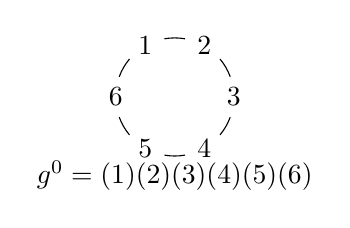
\begin{tikzpicture}
    \def \n {6}
    \def \radius {.75cm}
    \def \margin {20} % margin in angles, depends on the radius
    \node at (0,-1) {$g^0=(1)(2)(3)(4)(5)(6)$};
    \foreach \s in {1,...,\n}
    {
      \node at (-{360/\n * (\s - 3)}:\radius) {$\s$};
      \draw[-, >=latex] ({360/\n * (\s - 1)+\margin}:\radius) 
        arc ({360/\n * (\s - 1)+\margin}:{360/\n * (\s)-\margin}:\radius);
    }
\end{tikzpicture}
&
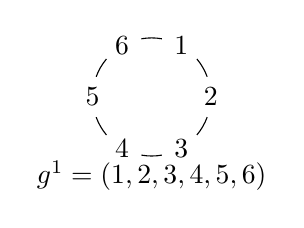
\begin{tikzpicture}
    \def \n {6}
    \def \radius {.75cm}
    \def \margin {20} % margin in angles, depends on the radius
    \node at (0,-1) {$g^1=(1,2,3,4,5,6)$};
    \foreach \s in {1,...,\n}
    {
      \node at (-{360/\n * (\s - 2)}:\radius) {$\s$};
      \draw[-, >=latex] ({360/\n * (\s - 1)+\margin}:\radius) 
        arc ({360/\n * (\s - 1)+\margin}:{360/\n * (\s)-\margin}:\radius);
    }
\end{tikzpicture}
&
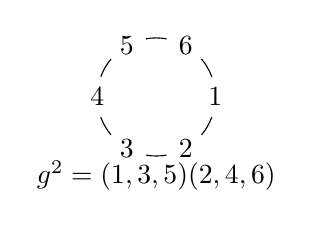
\begin{tikzpicture}
    \def \n {6}
    \def \radius {.75cm}
    \def \margin {20} % margin in angles, depends on the radius
    \node at (0,-1) {$g^2=(1,3,5)(2,4,6)$};
    \foreach \s in {1,...,\n}
    {
      \node at (-{360/\n * (\s - 1)}:\radius) {$\s$};
      \draw[-, >=latex] ({360/\n * (\s - 1)+\margin}:\radius) 
        arc ({360/\n * (\s - 1)+\margin}:{360/\n * (\s)-\margin}:\radius);
    }
\end{tikzpicture}
\\
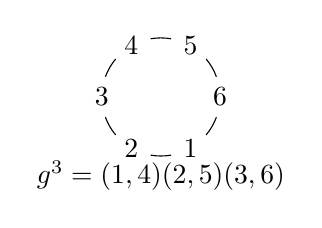
\begin{tikzpicture}
    \def \n {6}
    \def \radius {.75cm}
    \def \margin {20} % margin in angles, depends on the radius
    \node at (0,-1) {$g^3=(1,4)(2,5)(3,6)$};
    \foreach \s in {1,...,\n}
    {
      \node at (-{360/\n * (\s - 0)}:\radius) {$\s$};
      \draw[-, >=latex] ({360/\n * (\s - 1)+\margin}:\radius) 
        arc ({360/\n * (\s - 1)+\margin}:{360/\n * (\s)-\margin}:\radius);
    }
\end{tikzpicture}
&
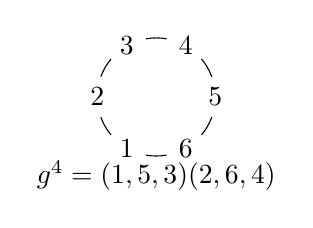
\begin{tikzpicture}
    \def \n {6}
    \def \radius {.75cm}
    \def \margin {20} % margin in angles, depends on the radius
    \node at (0,-1) {$g^4=(1,5,3)(2,6,4)$};
    \foreach \s in {1,...,\n}
    {
      \node at (-{360/\n * (\s + 1)}:\radius) {$\s$};
      \draw[-, >=latex] ({360/\n * (\s - 1)+\margin}:\radius) 
        arc ({360/\n * (\s - 1)+\margin}:{360/\n * (\s)-\margin}:\radius);
    }
\end{tikzpicture}
&
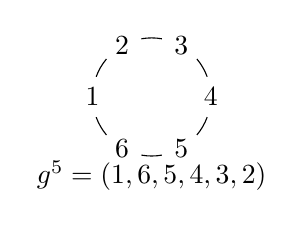
\begin{tikzpicture}
    \def \n {6}
    \def \radius {.75cm}
    \def \margin {20} % margin in angles, depends on the radius
    \node at (0,-1) {$g^5=(1,6,5,4,3,2)$};
    \foreach \s in {1,...,\n}
    {
      \node at (-{360/\n * (\s + 2)}:\radius) {$\s$};
      \draw[-, >=latex] ({360/\n * (\s - 1)+\margin}:\radius) 
        arc ({360/\n * (\s - 1)+\margin}:{360/\n * (\s)-\margin}:\radius);
    }
\end{tikzpicture}
\end{tabular}
\end{center}

\indent The cycle index polynomial is
\begin{equation*}
    Z_G=\frac{1}{6}(x_1^6+x_2^3+2x_3^2+2x_6)
\end{equation*}
where for $x^{i}_j$, $j$ is the length of each cycle, $i$ is the number of $j-cycles$, and the coefficient is the total group elements with this configuration. Plugging $2$ in for each $x_i$, we see that there are $14$ total arrangements.\\
\indent Now, let $Y$ be a set of colorings red and blue with weights $R$ and $B$ respectively. By P\'{o}lya's Theorem, the inventory of configurations $F(C)$ is 
\begin{align*}
    F(C) &= Z_G(R+B,R^2+B^2,\dots, R^6+B^6)\\
    &= \frac{1}{6}((R+B)^6+(R^2+B^2)^3+2(R^3+B^3)^2+2(R^6+B^6))\\
    &=R^6+R^5B+3R^4B^2+4R^3B^3+3R^2B^4+RB^5+B^6.
\end{align*}
From the term $4R^3B^3$, there are $4$ arrangements with $3$ red beads and $3$ blue beads. 
\end{exmp}

\begin{exmp}[Dihedral Necklaces]\hfill

What if we allow for flipping the necklaces? Suppose we have $6$ beads and $3$ colors, red, blue, and purple. We want to find out the total number of arrangements, as well as the number of arrangements with $2$ blue beads, $2$ red beads, and $2$ purple beads. We still consider two necklaces the same if they are cyclic rotations of each other, but now we also consider reflections. For example,
necklaces $RRBBPP$ and \reflectbox{$RRBBPP$} are the same. Let $X$ be the set of $6$ beads $X=\{1,2,\dots, 6\}$ and let $G$ be the \textit{dihedral group} of order $12$ that consists of rotations and reflections of $X$ such that $G=\{r^0,r^1,\dots r^5,s^0,s^1,\dots,s^5\}$ where $r^i$ are rotations and $s^i$ are symmetries (reflections). The rotations are listed in Example (\ref{necklace}), so we list the reflections:   
\end{exmp}

\begin{center}
\begin{tabular}{c c c}
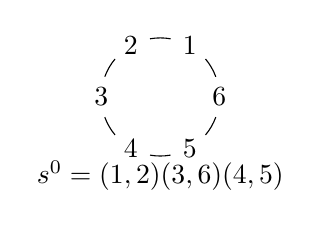
\begin{tikzpicture}
    \def \n {6}
    \def \radius {.75cm}
    \def \margin {20} % margin in angles, depends on the radius
    \node at (0,-1) {$s^0=(1,2)(3,6)(4,5)$};
    \foreach \s in {1,...,\n}
    {
      \node at ({360/\n * (\s)}:\radius) {$\s$};
      \draw[-, >=latex] ({360/\n * (\s - 1)+\margin}:\radius) 
        arc ({360/\n * (\s - 1)+\margin}:{360/\n * (\s)-\margin}:\radius);
    }
\end{tikzpicture}
&
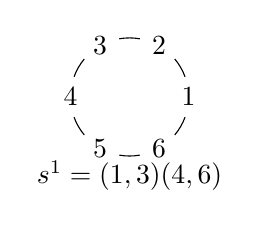
\begin{tikzpicture}
    \def \n {6}
    \def \radius {.75cm}
    \def \margin {20} % margin in angles, depends on the radius
    \node at (0,-1) {$s^1=(1,3)(4,6)$};
    \foreach \s in {1,...,\n}
    {
      \node at ({360/\n * (\s +5)}:\radius) {$\s$};
      \draw[-, >=latex] ({360/\n * (\s - 1)+\margin}:\radius) 
        arc ({360/\n * (\s - 1)+\margin}:{360/\n * (\s)-\margin}:\radius);
    }
\end{tikzpicture}
&
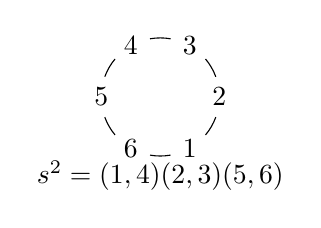
\begin{tikzpicture}
    \def \n {6}
    \def \radius {.75cm}
    \def \margin {20} % margin in angles, depends on the radius
    \node at (0,-1) {$s^2=(1,4)(2,3)(5,6)$};
    \foreach \s in {1,...,\n}
    {
      \node at ({360/\n * (\s+4)}:\radius) {$\s$};
      \draw[-, >=latex] ({360/\n * (\s - 1)+\margin}:\radius) 
        arc ({360/\n * (\s - 1)+\margin}:{360/\n * (\s)-\margin}:\radius);
    }
\end{tikzpicture}
\\
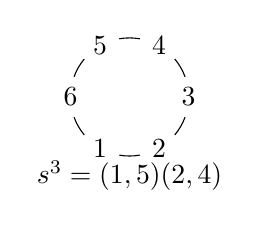
\begin{tikzpicture}
    \def \n {6}
    \def \radius {.75cm}
    \def \margin {20} % margin in angles, depends on the radius
    \node at (0,-1) {$s^3=(1,5)(2,4)$};
    \foreach \s in {1,...,\n}
    {
      \node at ({360/\n * (\s+3)}:\radius) {$\s$};
      \draw[-, >=latex] ({360/\n * (\s - 1)+\margin}:\radius) 
        arc ({360/\n * (\s - 1)+\margin}:{360/\n * (\s)-\margin}:\radius);
    }
\end{tikzpicture}
&
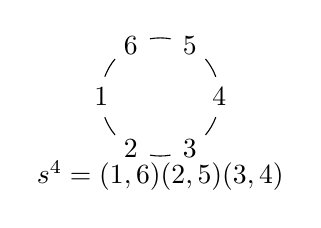
\begin{tikzpicture}
    \def \n {6}
    \def \radius {.75cm}
    \def \margin {20} % margin in angles, depends on the radius
    \node at (0,-1) {$s^4=(1,6)(2,5)(3,4)$};
    \foreach \s in {1,...,\n}
    {
      \node at ({360/\n * (\s+2)}:\radius) {$\s$};
      \draw[-, >=latex] ({360/\n * (\s - 1)+\margin}:\radius) 
        arc ({360/\n * (\s - 1)+\margin}:{360/\n * (\s)-\margin}:\radius);
    }
\end{tikzpicture}
&
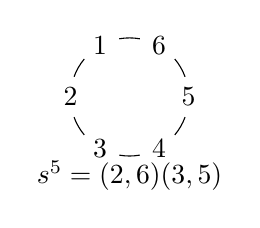
\begin{tikzpicture}
    \def \n {6}
    \def \radius {.75cm}
    \def \margin {20} % margin in angles, depends on the radius
    \node at (0,-1) {$s^5=(2,6)(3,5)$};
    \foreach \s in {1,...,\n}
    {
      \node at ({360/\n * (\s+1)}:\radius) {$\s$};
      \draw[-, >=latex] ({360/\n * (\s - 1)+\margin}:\radius) 
        arc ({360/\n * (\s - 1)+\margin}:{360/\n * (\s)-\margin}:\radius);
    }
\end{tikzpicture}
\end{tabular}
\end{center}

\indent The cycle index polynomial is 
\begin{equation*}
    Z_G=\frac{1}{12}(x_1^6 +3x_1^2x_2^2 + 4x_2^3 +2x_3^2 + 2x_6).
\end{equation*}
By plugging in $3$ for each $x_i$, we see that there are $92$ arrangements. Now, let $Y$ be a set of colorings red, blue, and purple, with weights $R$, $B$, and $P$ respectively. By P\'{o}lya's Theorem, the inventory of configurations $F(C)$ is 
\begin{multline*}
    F(C) = \frac{1}{12}((R+B+P)^6 + 3(R+B+P)^2(R^2+B^2+P^2)^2\\
             +4(R^2+B^2+P^2)^3 +2(R^3+B^3+P^3)^2 +2(R^6+B^6+P^6))
\end{multline*}

\begin{multline*}
    = B^6 +B^5R +3B^4R^2 +3B^3R^3 + B^2R^4 +BR^5 +R^6 +B^5Y +3B^4RP \\
     +6B^3R^2P + 6B^2R^3P + 3BR^4P + R^5P + 3B^4P^2 + 6B^3RP^2 + 11B^2R^2P^2  \\
     + 6BR^3P^2 +3R^4P^2 +3B^3P^3 +6B^2RP^3+3R^2P^4+BP^5+RP^5+P^6.
\end{multline*}
    The term $11B^2R^2P^2$ tells us there are $11$ arrangements with $2$ red beads, $2$ blue beads, and $2$ purple beads.
\section*{Acknowledgments}  
This paper would not have been possible without the help of many people. First, I would like to thank my mentor Adan Medrano Martin Del Campo for guiding me through the process. I would also like to thank my group members, Xifan Yu and Tianyi (Jerry) Zhang for listening to my presentations and giving me feedback. Lastly, I would like to thank Peter May for organizing the REU program.

\begin{thebibliography}{9}
\bibitem{Dummit and Foote}
Dummit, D. and Foote, R. \textit{Abstract Algebra}. 3rd ed. Wiley, New York, 2003.

\bibitem{Stanley}
Stanley, Richard (2011). \textit{Enumerative Combinatorics (2nd ed., Cambridge Studies in Advanced Mathematics)}. Cambridge: Cambridge University Press. doi:10.1017/CBO9781139058520

\bibitem{Bender}
E. A. Bender, \& J. R. Goldman. (1975). \textit{On the Applications of Mobius Inversion in Combinatorial Analysis}. The American Mathematical Monthly, 82(8), 789-803. doi:10.2307/2319793

\bibitem{Polya}
Gian-Carlo Rota
David A. Smith
\textit{Enumeration under group action}.
Annali della Scuola Normale Superiore di Pisa, Classe di Scienze 4e série, tome 4, no 4
(1977), p. 637-646

\bibitem{Algebraic Combinatorics}
Stanley, Richard (2013). \textit{Algebraic Combinatorics}. Version 1. Springer-Verlag New York, 2013.



\end{thebibliography}

\end{document}

